\chapter{Ladingsinjectie bij het gebruik van ideale SPICE bronnen.}
\label{app:chargeinj}
Bij het berekenen van de energie consumptie van verschillende bouwblokken, valt het op dat de voeding stroom opneemt i.p.v. levert bij het schakelen van de ideale spice bronnen. Dit komt door een ladingsinjectie van de ideale spice bronnen. Om dit te verifieren, worden de stromen van een simpele inverterschakeling bestudeerd. Figuur \ref{fig:chargeinj_inv} stelt een simple inverterschakeling voor met relevante parasitaire capaciteiten. Bij het aanleggen van een stapfunctie aan de inverter vloeit er een stroom door de capaciteiten. Omdat de positieve stroom die geobserveerd wordt in de voeding afkomstig is van de ingang, moet de som van de stromen door de ingang, voeding en grond nul zijn. De stroom door de ingang kan in SPICE opgemeten worden door een weerstand met resistieve waarde gelijk aan nul, in serie met de ingang te zetten.\\
Figure \ref{fig:chargeinj_cur} toont deze drie stromen. In het eerste deel van de figuur (tot tijdstip 30ps) is de spanning aan de input al aan het stijgen maar de invertor is nog niet aangeschakeld. De voedings- en grondstromen komen dan puur van de ingang. Vanaf tijdstip 30ps, is de invertor aan het schakelen en is er een aandeel van de stroom in de grond die afkomstig van de voeding is. De som van de drie stromen is ten alle tijden gelijk aan nul.
We kunnen dus besluiten dat er een ladingsinjectie is van ideale spice bronnen in het circuit. Dit heeft een invloed op de stromen en daardoor ook op de energie berekeningen, maar dit verwaarlozen we bij onze berekeningen.

\begin{figure}[!ht]
  \centering
  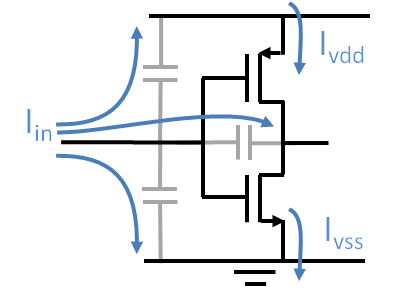
\includegraphics[width=0.4\textwidth]{../fig/hfdst-chargeinj-inv.png}
  \caption[Ladingsinjectie: testcircuit]{Testcircuit ladingsinjectie}
  \label{fig:chargeinj_inv}
\end{figure}

\begin{figure}[!ht]
  \centering
  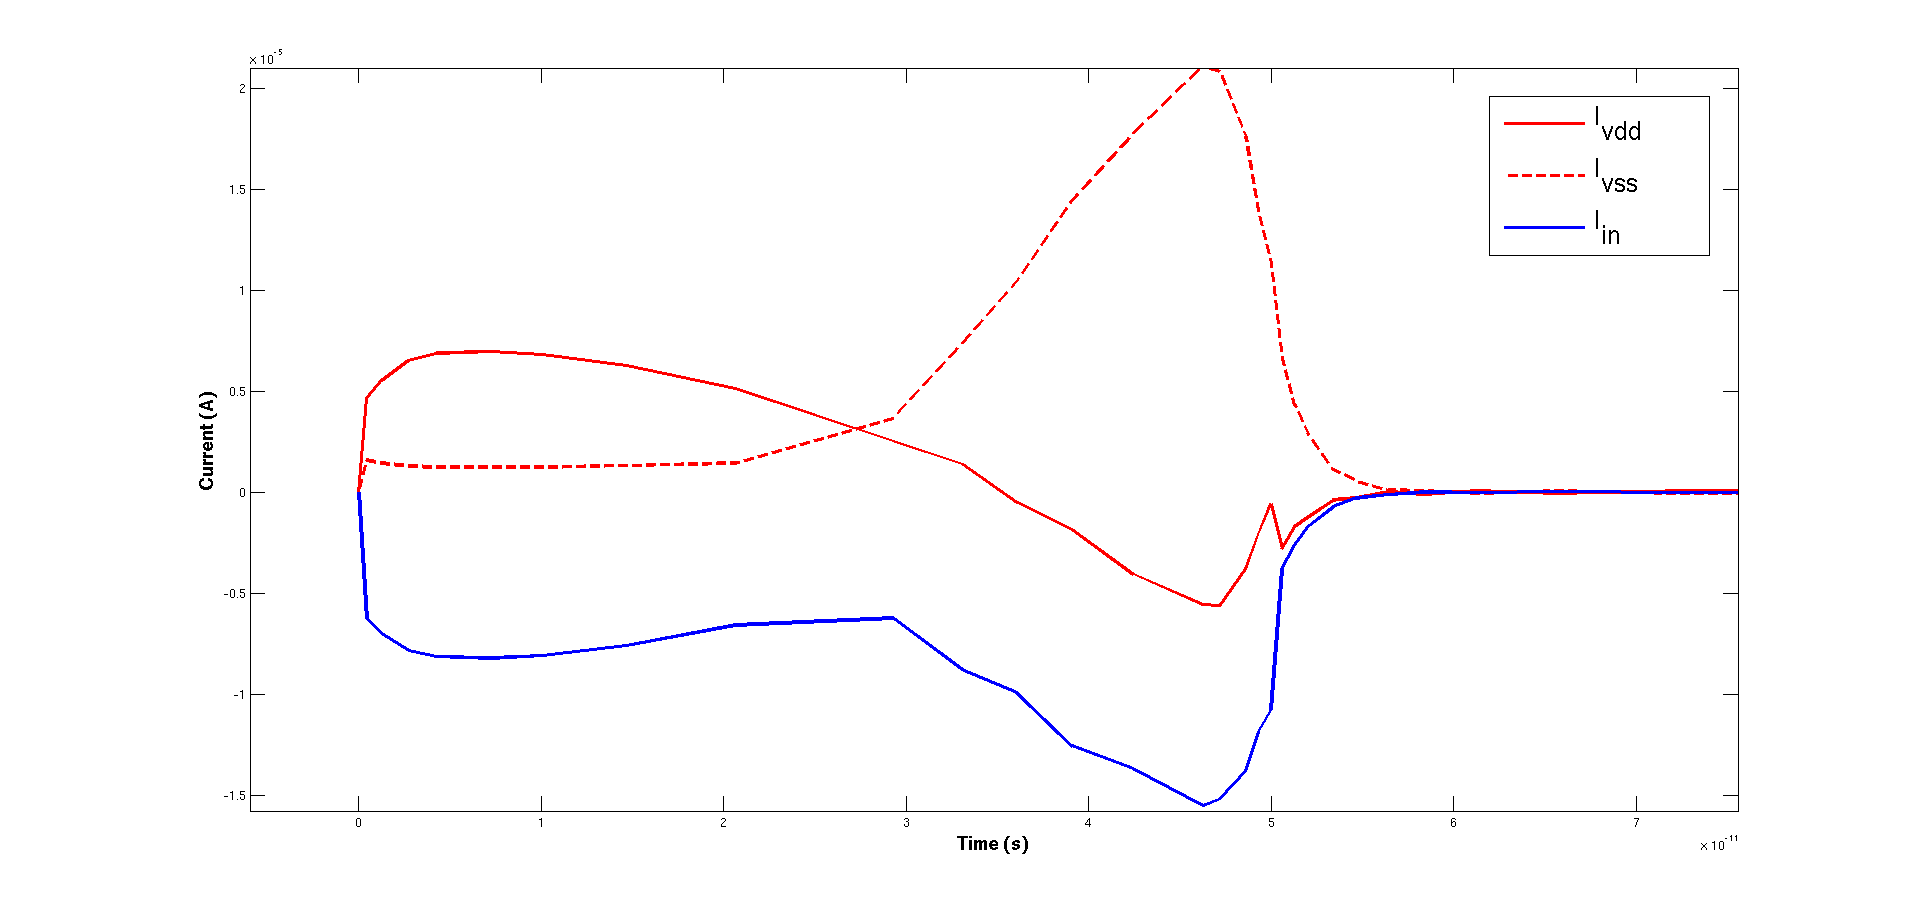
\includegraphics[width=\textwidth]{../fig/hfdst-chargeinj-currents.png}
  \caption[Ladingsinjectie: stroom]{Stromen in circuit}
  \label{fig:chargeinj_cur}
\end{figure}
